%% $RCSfile: proj_proposal.tex,v $
%% $Revision: 1.2 $
%% $Date: 2010/04/23 02:40:16 $
%% $Author: kevin $

\documentclass[11pt, a4paper, notitlepage]{article}
\usepackage{tabularx}
\usepackage{float} % lets you have non-floating floats
\usepackage{cite}
\usepackage{url} % for typesetting urls


%  We don't want figures to float so we define
%
%\newfloat{fig}{thp}{lof}[section]
\floatname{fig}{Figure}




%% These are standard LaTeX definitions for the document
%%
\title{Web Application Key Management Progress Report}
\author{Sriram Venkatesh}

%% This file can be used for creating a wide range of reports
%%  across various Schools
%%
%% Set up some things, mostly for the front page, for your specific document
%
% Current options are:
% [ecs|msor]              Which school you are in.
%
% [bschonscomp|mcompsci]  Which degree you are doing
%                          You can also specify any other degree by name
%                          (see below)
% [font|image]            Use a font or an image for the VUW logo
%                          The font option will only work on ECS systems
%
\usepackage[image,ecs]{vuwproject} 

% You should specifiy your supervisor here with
%     \supervisor{Firstname Lastname}
% use \supervisors if there are more than one supervisor

% Unless you've used the bschonscomp or mcompsci
%  options above use
\otherdegree{Bachelor of Engineering}
% here to specify degree

\supervisors{Dr Ian Welch, Michael Gannon,  Nick Clarke, Dr Kris Bubendorfer}


% Comment this out if you want the date printed.
\date{}

\begin{document}

% Make the page numbering roman, until after the contents, etc.
\frontmatter

%%%%%%%%%%%%%%%%%%%%%%%%%%%%%%%%%%%%%%%%%%%%%%%%%%%%%%%

\begin{abstract}
The objective of this report is describe and demonstrate the progress of the Web Application Key Management project and develop a plan for the remainder of the project. The project looks at how applications can manage encrypted credential keys for secure web applications. The project is split into two phases, where we look into the traditional case and also a modern case of moving the application into the cloud. The literature review conducted finds there have been various attempts to solve the issue. This report looks at a comparative view of the best option by comparing various threat models and abstractions. 
\end{abstract}

%%%%%%%%%%%%%%%%%%%%%%%%%%%%%%%%%%%%%%%%%%%%%%%%%%%%%%%

\maketitle

%\tableofcontents

% we want a list of the figures we defined
%\listof{fig}{Figures}

%%%%%%%%%%%%%%%%%%%%%%%%%%%%%%%%%%%%%%%%%%%%%%%%%%%%%%%

\mainmatter

%%%%%%%%%%%%%%%%%%%%%%%%%%%%%%%%%%%%%%%%%%%%%%%%%%%%%%%

\section{Introduction}
As the web becomes increasingly complex, web applications become more complicated and dynamic. Web pages are no longer static; they contain dynamic content from many different external sources such as external data stores or web services. To access these external services, the web application is configured with credentials to gain access to those systems. The credentials used can be username and password pairs, certificates or even the use of API Keys. If an attacker compromises the web application or any component of the system, we want to make it difficult for them to steal the secret credentials and gain access to those external systems. Given this threat, we need a proper management system that can securely manage these security credentials throughout the application life cycle. \\

This project explores this concept of manging these secrets and analyzes the solution into two main phases. The first phase analyzes the traditional situation, with a local physical server that we control. While the second phase of the project looks into how we can manage the secrets when we move the application into the cloud. This preliminary progress report has a major focus on the first phase of the project. 

\subsection*{Key Management}
The core problem I am investigating in this project is the difficulty of ensuring secure key management. Key management is a broad concept used to define the secure management of secret keys or credentials. Leakage of these of secrets can have hazardous social and monetary implications \cite{huang2003web}. These valuable keys need to be securely managed and have proper authorization mechanisms to ensure that key external services are not compromised. 

In this project we analyze the problem of key management via three main high level objectives.

\begin{enumerate}
\item \textbf{Secure Key Management} \\
A secure key management plan needs to ensure that keys are secure throughout the life cycle of the web application. This involves how it generates the keys at boot, and how to destroys any keys during the shutdown of these services \cite{entrprise-guide}. The application also requires the key for it to be able to decrypt the data at runtime. 

\item \textbf{Secure Key Storage} \\
Keys must be securely stored throughout their operational life. The key should be placed in a secure storage and details around how the keys are protected evolve around the web application  \cite{entrprise-guide}. 

\item \textbf{Key Usage Authorization} \\
Measures must be implemented to ensure that keys can be used only for authorized  purposes by authorized entities and that authorized access to keys cannot be interrupted by others  \cite{entrprise-guide}. Control of access, authentication of users and confidentiality protection are all critical to meeting this objective.
\end{enumerate}

\makeblankpage


\section{Background}
This section describes different key management models and algorithms that could be applied to this project. However, before the key management models and algorithms are described, it is necessary to provide a general introduction into computer security. 

\subsection*{System Security}
Before someone can determine whether something is secure or not, we have to first create a baseline for what is a \emph{secure} system. In computer security, a typical approach is to require confidentiality, integrity, access control, availability, authentication and non-repudiation in the system\cite{Pfleeger:2006:SC:1177321}. \\

These six attributes are described as follows:

\begin{enumerate}
\item \textbf{Confidentiality} is to ensure that secret information is never disclosed to unauthorized entities.
\item \textbf{Access Control} is to ensure that authorized entities are granted permissions to the resource.
\item \textbf{Integrity} is to ensure that data will not be corrupted.
\item \textbf{Availability} is a guarantee of accessibility of data in the system.
\item \textbf{Authentication} is the ability to verify the identity of an entity.
\item \textbf{Non-repudiation} means that one cannot claim that certain actions were never performed. For example, if a message is transmitted or the act of signing the message.
\end{enumerate}

Although it is important to consider all these security attributes when designing a web application, its not always possible or necessarily required that all six attributes be fulfilled completely. 

\subsection*{Cryptographic Basics}
The basic aim of \emph{cryptography} is to enable two people to communicate over an insecure channel in a secure way. The term cryptography describes a range of cryptographic services including techniques for providing both confidentiality and authentication. 

\subsubsection*{Symmetric Encryption}
Symmetric Encryption, has a single secret key that it can use to encrypt plaintext. Then using the same secret key another user can decrypt it \cite{ferguson2003practical}. Symmetric key encryption is an essential mechanism for protecting data at rest. We can use this to reduce the risk of unauthorized access to sensitive data. However, the use of symmetric key encryption brings with it certain dangers. Most important is that, once encrypted, we need a robust mechanism to ensure the encryption key is protected from unauthorized access. The key management system needs to grant access to trust worthy entities, and restrict unauthorized entities to ensure that the key is secure. 

\subsubsection*{Asymmetric Cryptography}
Asymmetric Cryptography is a cryptographic algorithm which requires two separate keys, one of which is private and one which is public \cite{ferguson2003practical}.
The public and private key pair comprise of two uniquely related cryptographic keys. The public key is made available to everyone via a publicly accessible repository or directory. While on the other hand the private key must remain \emph{confidential} to its respective owner. Because the key pair is mathematically related, the public key is used to encrypt the \emph{plaintext}, whereas the private key is used to decrypt the \emph{ciphertext} produced by the public key. Therefore, Asymmetric cryptography can provide confidentiality, as the user with the private key is only one able to decrypt the message \cite{pub-key}.

\subsection*{Basic Key Management}
Encryption Key Management is the administration of tasks involved with protecting, storing, backing up and organizing encryption keys or secrets. \cite{defination:key-management}. It considers the general management of cryptographic keys, and the means by which public keys are distributed. The study of key management can be broken down into phases concerning the life-cycle of a cryptographic key. These four phases are: \\

\begin{enumerate}
\item \textbf{Key Generation} which covers the creation of the keys
\item \textbf{Key Establishment} which is the methods by which the keys are distributed to the relevant users in the network.
\item \textbf{Key Update} which the techniques used to renew or refresh the keys in the system 
\item \textbf{Key Destruction} which covers the deletion and disposal of keys when they are no longer of use.
\end{enumerate}

Establishing and distributing keys over an unsecured channel is an important consideration to make. An elegant and widely-applied scheme for establishing a shared key across an insecure channel is the \emph{Diffie-Hellman} key exchange. The Diffie-Hellman key exchange is a specific method of exchanging cryptographic keys. The Diffie-Hellman key exchange method allows two parties that have no prior knowledge of each other to jointly establish a shared secret key over an insecure communication channel. \\


\subsection*{Public Key Infrastructure (PKI)}
A public key infrastructure (PKI) is a set of hardware, software and procedures needed to manage and distribute digital certificates. The aim of PKI is to provide confidentiality, integrity, access control and authentication \cite{PKI:Online}. \\

There are different types of systems in a PKI:
\begin{itemize}
\item \textbf{Private and Public Key Systems:} Private systems are symmetric cryptography and a public systems are asymmetric cryptography. Currently, public key systems are the most common.
\item \textbf{Symmetric Encryption Systems:} The same key is used for both the processes of encryption and decryption.
\item \textbf{Asymmetric Encryption Systems:} A different key is used for each process. One key is the public key and the other key is the private key. If something is encrypted with the public key, then decryption can only be done with the private key. Alternatively, if something is encrypted with the private key, then decryption must be done only with the public key.
\end{itemize}

A certificate authority (CA) is the entity providing the keys. The private key will be given to the person requesting the key. The public key is made public in a directory for users. No one can ever find out what someone’s private key is, never being available on the Internet. The private key is used for proving user identity and encrypting the digital certificate. The digital certificate will be decrypted by the public key, which is used by the message receiver. \cite{PKI:Online}


\subsection*{Interoperability Standards}
\subsubsection*{Public Key Cryptography Standard \#11 (PKCS\#11)}
Public Key Cryptography Standard \#11  (PKCS \#11) specifies an API for cryptographic devices that is widely adopted in industry. PKCS \#11 defines a platform-independent API to cryptographic tokens, which is called \emph{"Cryptoki"} \cite{bortolozzo2010attacking}. The PCKS \#11 was not intended to be a general interface to cryptographic operations, it was rather used to build such services \cite{p}.

\subsubsection*{Key Management Interoperability Protocol (KMIP)}
The Key Management Interoperability Protocol (KMIP) is a communication protocol between key management systems and encryption systems. The KMIP standard is controlled by the Organization for the Advancement of Structured Information Standards (OASIS). \\

KMIP does not include any specification or description of a key management framework or infrastructure. The problem addressed by KMIP is primarily that of standardizing communication between cryptographic clients that need to use the keys and key management systems that generate and manage those keys. Therefore, web application developers will be able to deploy a single key management infrastructure to manage keys for the different types of keys in different applications. \\


Many credential management systems have been developed in order to protect and secure the valuable credential data. Much of the research conducted in this project is about finding ways to address the problems associated with key management, and finding a solution so that we may securely manage credential data. \\

\subsection*{Trust Management Systems}
A trust management system provides a standard, general-purpose mechanism for specifying application security polices and credentials. The credentials are bound to public keys, which are authorized to perform specific tasks such as connecting to a database. \cite{blaze1999keynote}. \\

Trust management systems were devised as a alternative to Access Control Lists (ACL). An ACL, is a list of permissions attached to an object. It will specify what users, or system processes are granted access to objects, and also specify what operations are allowed on given objects. \cite{acl-rfc} These system need to grant or restrict access to resources according to some security policy. \\

One of the core problems of key management is Authorization. Using an Access Control List on a particular key or secret we can verify if the calling process is allowed to read the secret. We want to make sure that only verified processes should be granted access to the secret. A trust management system may be applicable, here has the entities want to engage in trust-requiring transaction.\cite{herzberg2000access} \\


\subsubsection*{Kerberos}
Kerberos can be viewed as a security system that assists clients in setting up a secure channel with any server that is part of a distributed system. Security is based on shared secret keys. There are two different components: 
\begin{itemize}
\item \textbf{Authentication Server (AS)} is responsible for handling a login request from a user. The AS authenticates a user and provides a key that can be used to set up secure channels with servers.
\item \textbf{Ticket Granting Service (TGS)} hands out specific messages, known as tickets, that are used to convince a server that the client is really who he claims to be.
\end{itemize}

\makeblankpage

\section{Project Progress}
The first phase of the project is to analyze and threat model the web application in the traditional case, and provide suitable recommendations and risks associated with it. I have applied the OWASP Threat Modeling Methodology. \cite{threat-modelling-owasp}\\

Threat modeling is an approach for analyzing the security of an application. It is a structured approach that enables you to identify, quantify, and address the security risks associated with an application. The OWASP Threat Modeling methodology involves applying the following steps to model the application: 

\begin{itemize}
  \item Create use cases to understand how the application is used.
  \item Identify the Entry Points to see where a potential attacker could interact with the application.
  \item Identify Assets that the attacker would be interested in.
  \item Identify assumptions for the components of the application, that an attacker would be interested in.
  \item Identify trust levels which represent the access rights the application with grant to external entities. 
\end{itemize}

\subsection*{Description of the Baseline Model}
The traditional case involves a local physical server that we control. The web application is hosted on this server and it needs access to an external datastore. For this case, we are using a Tomcat Container to host the application's Java code. The password is stored in \emph{plain-text} in a configuration file on disk. Even if we encrypt the stored password here, we will have the same problem of securing the encryption key, so we have simplified the case here.\\

\begin{figure}[h]
    \centering
    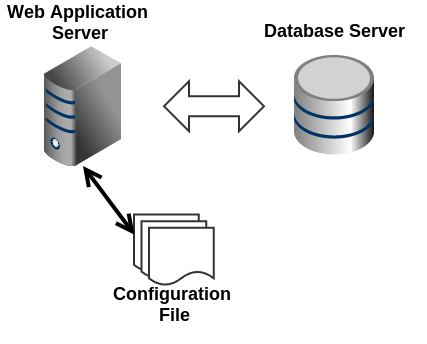
\includegraphics[width=0.5\textwidth]{config}
    \caption{Connection between application, database and configuration file}
\end{figure}

\makeblankpage

\subsection*{Decoupling the Application}

\subsubsection*{Actors of the Application}
Our application is made of various internal components that are involved with the credential  information that we want to protect. 
\begin{itemize}
	\item \textbf {Web Browser} \\
	The User using the web application from the external source
	\item \textbf{Web Application} \\
	The web application is the application that is run on top of the tomcat container. The web application itself as distinct from the Tomcat container software.
	\item \textbf{Tomcat Container} \\
	The Tomcat container is Tomcat process that runs the Web application code
	\item \textbf{Java Process/Java Virtual Machine} \\
	The Tomcat servlet is run on top of a JVM. The code is compiled and the resulting bytecode is run within the JVM.
	\item \textbf {Operating System} \\
	The operating system is an abstracted layer that allows processes above to request for resources lower in the system such as memory or files on disk. The operating system has two layers.
	\begin{itemize}
		\item \textbf {Operating System User Accounts } \\
		The different user accounts associated with the operating system. These are processes which are run under the user. 
		\item \textbf {Operating System Facilities } \\
		The operating system has  the ability to make system calls to the via
		the OS kernel only
	\end{itemize}
\end{itemize}


\subsubsection*{Users Roles of the Application}
The configuration file needs to be protected via ACLs to ensure authorized access. Before defining the policy, its important to highlight the involved users in the application. The following user roles are involved with the application:
\begin{itemize}
\item \textbf{Tomcat Account}: The tomcat account is the limited account that runs the tomcat processes including the JVM process. 
\item \textbf{Root User}: The root user is the user that superuser account that has full access to the system. These users have elevated privileges on the system to configure and management the system
\item \textbf{Administrators of the Tomcat}: These are the users who administrate the tomcat container and also have access to the deployment details.
\end{itemize}

\subsubsection*{Trust Model Assumptions}
\begin{itemize}
\item We assume that the connection between the Application Server and Database is secure.
\end{itemize}

\subsection*{Interaction Between Components}
\subsection*{Running Application}
The running application requires the \emph{plain-text} password for the connection to occur. The following steps occur during the runtime of the application to obtain the \emph{plain-text} password from the file on disk. 

\begin{enumerate}
\item When the password is required for the database connection, the Java code executes a JDK method to read a file. This is executed when the tomcat instance runs the complied servlet code.
\item This JDK method will be abstracted to a system call, which will tell the operating system to read that file. 
\item The operating system finds the location of the file and verifies whether the calling process is allowed access to the file.
\item Once, the operating system verifies the process, the operating system will obtain a copy of the configuration file on disk and put into memory for the Java process to access.
\item The Java process will process the reference in memory of the configuration file and extract the password required to connect to the datastore.
\end{enumerate}


\subsection*{Threat Scenarios}
After completing the analysis above, we can slowly see the different entities and users involved with the application and how it manages its credentials. We can now generate a list of threat scenarios that affect the application's secrets if an attacker where to compromise the entity. \\

\begin{itemize}
\item If an attacker is able to inject code into the system via the web browser entry point, it will be executed as the tomcat process. This can be proved to be dangerous because the tomcat process has read access to the file and knows the location of the encryption on key. Armed with both of these tools. After getting to this information, the attacker can use this data to connect the external system. This is problematic because its difficult to figure out if the legitimate tomcat process is requesting the data or the attacker because the attacker is hidden by the facade of the tomcat process.
\item Given an attacker has access to the JVM. Any code that is executed as the JVM is executed as the tomcat precess as well. Which means given the attacker can run code or view the complied class file, the attacker is able read the secret
\item Given an web browser is given access to more files other than the webroot. It means the attacker is able to view important configuration data, which may involve the configuration data. 
\item Once the attacker has control of the hard disk. The attacker is able to read the configuration file and read the secret.
\item If an attacker is able to deploy tomcat applications. He will have the capability to run applications that request for the password from the configuration file. As the system does not differentiate between different applications it will be hard to ensure that the secrets will be safe.
\item If the attacker is able to gain access to either Root or Tomcat Process, in the operating system later of the application, the attacker will be allowed to execute arbitrary  commands which inturn can reveal secret.
\item If the attacker is able to gain access to a user account on system that allows him to read contents of files visible to Operating System Tomcat user account. he will be able to read the configuration data.
\end{itemize} 


\section{Working Plan}
\subsection*{Future Stages}
The main components remaining for the first phase of the project include designing, implementation and evaluation of the first phase. While the designing and implementation of the second phase of the project has not yet started. An additional project analysis of the baseline model, has been added to the project phase to gain clarity of the project aims and goals. This has slightly shifted the timeline of the project as seen in Figure~\ref{gantt}

\begin{figure}[h!]
    \centering
    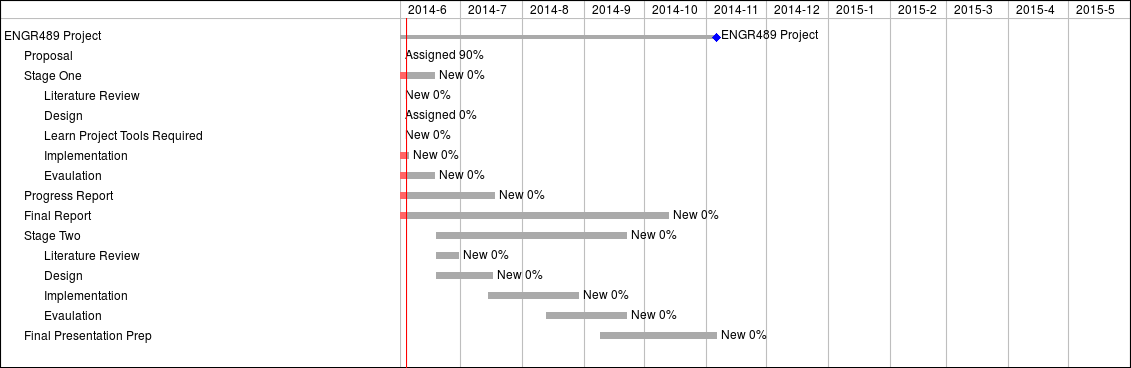
\includegraphics[width=0.95\textwidth]{gannt.png}
    \caption{Gantt Chart}
    \label{gantt}
\end{figure}

\subsection*{Evaluation}
After designing and implementing a solution, how do we evaluated the better solution between the different key management models. Following a similar process, used above, a threat model will be crafted around the implementation detailing:
\begin{itemize}
\item Decouple the solution
\item The boundaries of trust between the different entities
\item Generate Threat Scenarios based on assumptions at each entity
\item Rank the threat in terms of impact and damage on the application
\end{itemize}

\subsection*{Feedback Requested}
The following feedback would be greatly appreciated and helpful for the second half of the project.

\begin{itemize}
\item Comments on evaluation plan that has been outlined.
\item Comments regarding threats generated in section 4.
\end{itemize}



%%%%%%%%%%%%%%%%%%%%%%%%%%%%%%%%%%%%%%%%%%%%%%%%%%%%%%%
\backmatter
%%%%%%%%%%%%%%%%%%%%%%%%%%%%%%%%%%%%%%%%%%%%%%%%%%%%%%%

\bibliographystyle{ieeetr}
\bibliography{bib}

\end{document}
